The dataset was constructed by sampling from two Gaussian distributions with
equal covariance but different means. A non-stationary perturbation
in feature space was generated with the Laplace distribution function
\begin{align} \label{eq:laplace_dist}
  f(x \vert \mu, b) = \frac{1}{2b} e^{-\frac{\lvert x - \mu\rvert}{b}},
\end{align}
with $b=9$ and $\mu=60$, where the argument $x$ is the position in the dataset.
This makes the instances non-\ac{IID} (see Figure~\ref{fig:artdata}), with a known dispersion function.

\begin{figure}
  \center
  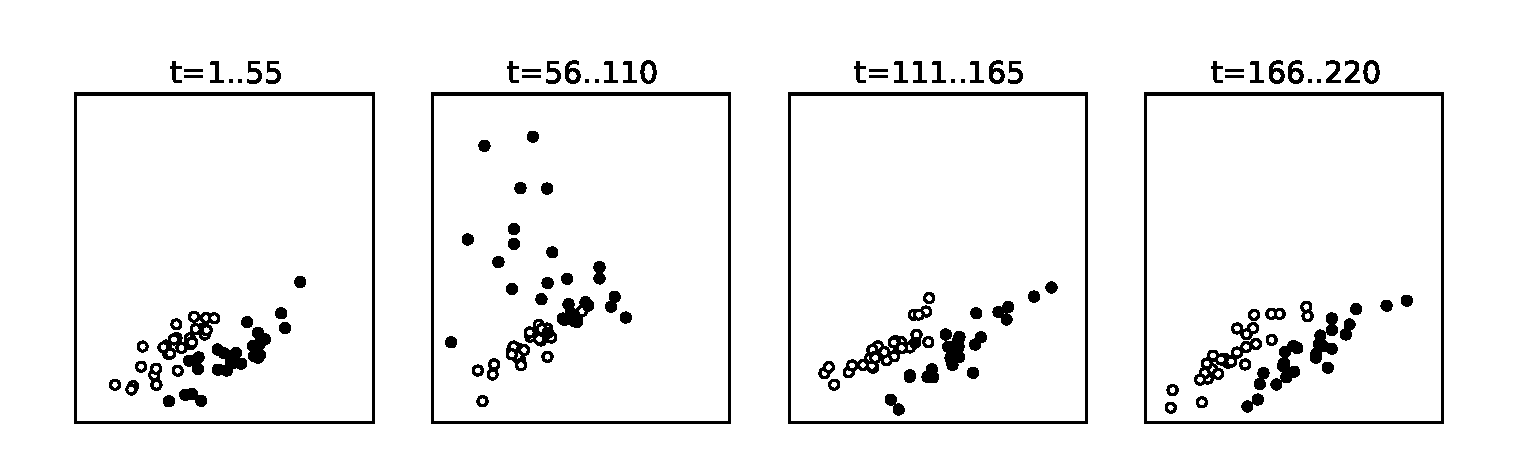
\includegraphics[width=\textwidth]{artdata.pdf}
  \caption{Sequential snapshots of the artificial dataset used to evaluate the
    \protect\ac{dSVM}. The data is sampled form two Gaussian distributions with
    different means but equal covariance. In the second frame, we introduce a
    latent error, that leaks to a range of related of samples.}
  \label{fig:artdata}
\end{figure}

A Laplace distribution was chosen based on its similarity to the empirical
distribution found in a preliminary experiment, in which we modeled the
interdependence of slack variables in the training set of a \ac{BCI}
experiment. As the strongest dependence in this preliminary experiment was
found between slack variables of the same class, the perturbation was limited
to one class only.

\begin{sloppypar}
Both a soft-margin \ac{SVM} and a \ac{dSVM} were trained on this artificially
constructed dataset. Model selection for the cost parameter $c$ was performed
with a line search on cross-validated accuracy with four sequential subsets
corresponding to the frames in Figure~\ref{fig:artdata}. The \ac{dSVM}'s
dispersion matrix $D$ was constructed using \eqref{eq:laplace_dist}:
%
\begin{align} \label{eq:dfunc}
  \tilde{D}_{i,j} &=
    \begin{cases}
      \vec{g}_i \cdot f(\lvert \vec{t}_i - \vec{t}_j \rvert) 
        & \text{if } \vec{y}_i = \vec{y}_j,
    \\
      0 & \text{otherwise}
    \end{cases}
\end{align}
where $\vec{t}_i$ is the time offset of an instance, and $\vec{g}$ chosen such
that the columns of $D$ are normalized to one.
\end{sloppypar}

\begin{figure}
  \center
  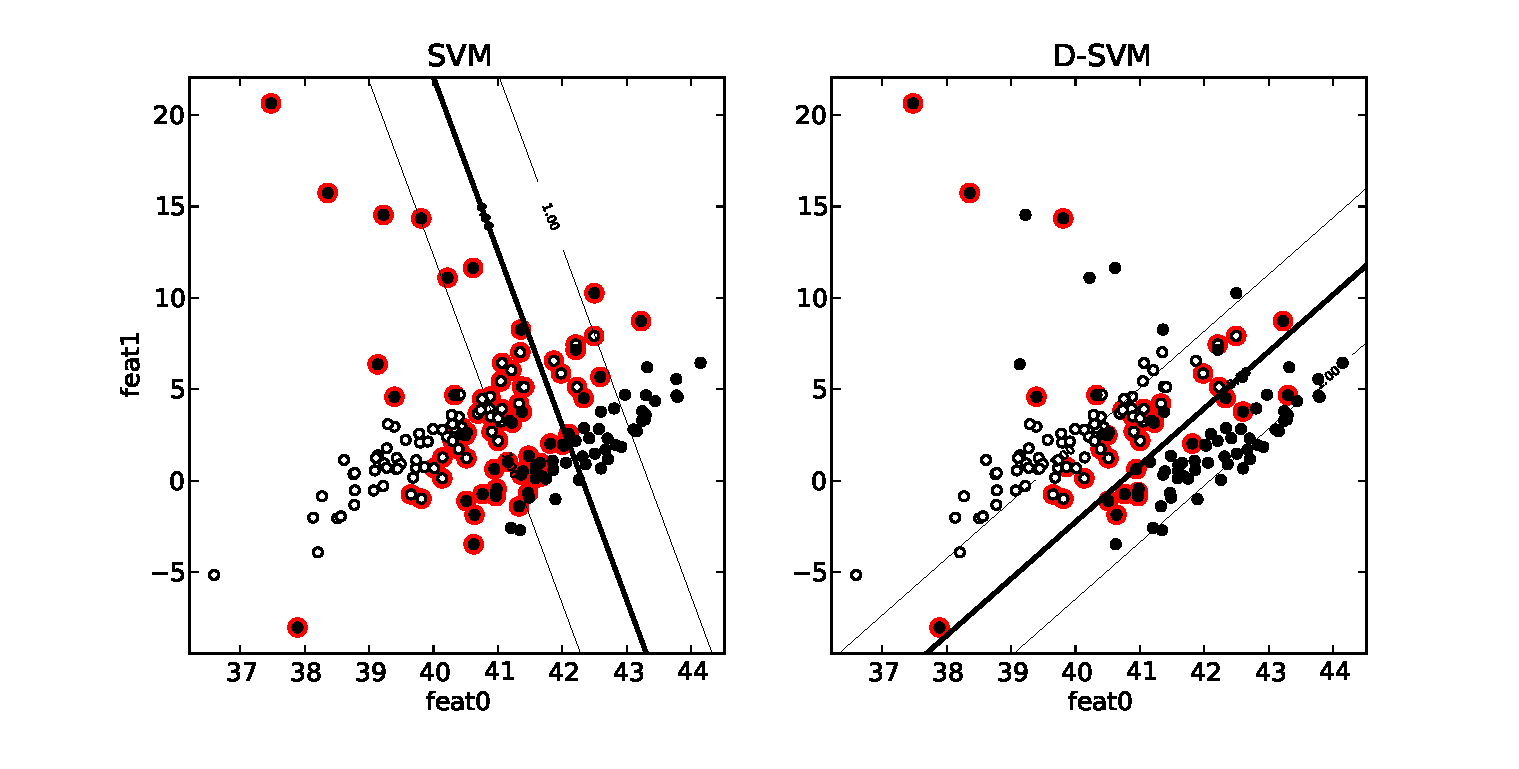
\includegraphics[width=\textwidth]{svm_vs_dsvm.pdf}
  \caption{The hyperplane (thick black line) and margin (between the thin black
    lines) for the standard soft-margin \protect\ac{SVM} (left) and the
    \protect{dSVM} (right). Both classifiers were trained on the artificial data
    displayed in Figure~\ref{fig:artdata}. The two classes are indicated with
    white and black dots respectively, red edges indicate the support vectors.
    While the dependent outliers displace the hyperplane of the standard
    \protect\ac{SVM}, the \protect\ac{dSVM} is able to reduce the weight of
    these points based on their relatedness.}
  \label{fig:svm_vs_dsvm}
\end{figure}

The resulting margins and hyperplanes are displayed in
Figure~\ref{fig:svm_vs_dsvm}. It can be seen that the soft-margin \ac{SVM} was
sensitive to the outliers produced by our non-stationary perturbation, with the
result that the hyperplane was almost orthogonal to the hyperplane that would
separate the two Gaussian distributions. In contrast, the \ac{dSVM} was able to
exploit the known dependence between the training instances, and separated the
two Gaussian distributions correctly in the presence of the perturbation. This
demonstrates how the \ac{dSVM} can use dependency information to avoid
overfitting if the training data is non-\ac{IID}.
